% !TEX root = thesis.tex
\documentclass[12pt,a4paper,titlepage,listof=totoc,bibliography=totoc,chapteratlists=0pt]{scrreprt}
\newcommand{\thesislang}{de} % en or de
\newcommand{\thesistitle}{Unser Thema ist Next Level}
\newcommand{\department}{Informatik} % Replace with your department

\newcommand{\firstauthor}{Stefan Schwammal}
\newcommand{\secondauthor}{Stefanie Schwammal}
\newcommand{\thirdauthor}{Sabine Schwammal}
\newcommand{\fourthauthor}{Sebastian Schwammal}

\newcommand{\duedateen}{April 4, 2025} % due date in English format
\newcommand{\duedatede}{4. April 2025} % due date in German format
\newcommand{\supervisor}{Lukas Lehrer}
\newcommand{\projectpartner}{Petra Programmierer, Initech Inc.}
\begin{filecontents*}{\jobname.xmpdata}
	\Keywords{VR, IOT, TODO}
	\Title{Unser tolles Thema -- wir sind suppa}
	\Author{Stefan Schwammal, Susi Schwammal}
\end{filecontents*}

\setcounter{tocdepth}{1}

\usepackage[utf8]{inputenc}
\usepackage[T1]{fontenc}
\usepackage{amsmath}
\usepackage{amsfonts}
\usepackage{amssymb}
\usepackage[table]{xcolor}
\usepackage{graphicx}
\usepackage[left=3.50cm, right=2.00cm, top=2.00cm, bottom=2.00cm,foot=1cm]{geometry}
\usepackage[splitrule,hang,flushmargin,multiple,bottom]{footmisc}
\usepackage{lmodern, textcomp}
\usepackage{lmodern}
\usepackage{pdfpages}
\usepackage[ngerman]{babel}
\usepackage{multicol}
\usepackage{float}
\usepackage{array,tabularx,booktabs}
\usepackage{ragged2e}
\usepackage{lipsum}
\usepackage{wrapfig}

\newcolumntype{M}[1]{>{\centering\arraybackslash}m{#1}}

\usepackage{enumitem}
\newlist{compactitem}{itemize}{3}
\setlist[compactitem,1]{label=\textbullet, nosep,leftmargin=1.5em,labelwidth=*,align=left}
\setlist[compactitem,2]{label=--, nosep,leftmargin=1.5em,labelwidth=*,align=left}
\setlist[compactitem,3]{label=\textopenbullet, nosep,leftmargin=1.5em,labelwidth=*,align=left}
\newlist{compactenum}{enumerate}{3}
\setlist[compactenum,1]{label=\arabic*., nosep,leftmargin=1.5em,labelwidth=*,align=left}
\setlist[compactenum,2]{label=\alph*., nosep,leftmargin=1.5em,labelwidth=*,align=left}
\setlist[compactenum,3]{label=\roman*., nosep,leftmargin=1.5em,labelwidth=*,align=left}
\newlist{compactdesc}{description}{3}
\setlist[compactdesc]{leftmargin=1.5em,labelwidth=*,align=left}

\usepackage{microtype}

\usepackage[parfill]{parskip}

\definecolor{bluekeywords}{rgb}{0.13,0.13,1}
\definecolor{greencomments}{rgb}{0,0.5,0}
\definecolor{redstrings}{rgb}{0.9,0,0}
\definecolor{lightgray}{gray}{0.9}
\definecolor{lightblue}{rgb}{0.93,0.95,1.0}

\usepackage{listings}

\makeatletter
\lstdefinestyle{lststyle}{
	basicstyle=%
	\ttfamily
	\lst@ifdisplaystyle\scriptsize\fi
}
\makeatother

\renewcommand{\lstlistlistingname}{List of Listings}
% TODO: define other languages as needed
\lstset{language=Python,
numbers=left,               
numberstyle=\tiny,          
showspaces=false,
showtabs=false,
breaklines=true,
lineskip=-1pt,
tabsize=2,
showstringspaces=false,
breakatwhitespace=true,
escapeinside={(*@}{@*)},
commentstyle=\color{greencomments},
keywordstyle=\color{bluekeywords}\bfseries,
stringstyle=\color{redstrings},
style=lststyle,
xleftmargin=17pt,
         framexleftmargin=17pt,
         framexrightmargin=5pt,
         framexbottommargin=4pt
}
\lstset{
morekeywords={base,var,in,out,dynamic,from,where,select,orderby,function,\$,group,by,into,yield,async,await,@,None,self,as,elif,with}
}
\lstdefinelanguage{TypeScript}{
	keywords={typeof, new, true, false, catch, function, return, null, switch, var, if, in, while, do, else, case, break, void, number, string, boolean, module, \$, export, for, this},
	keywordstyle=\color{blue}\bfseries,
	ndkeywords={class, export, boolean, throw, implements, import, this},
	ndkeywordstyle=\color{darkgray}\bfseries,
	identifierstyle=\color{black},
	sensitive=false,
	comment=[l]{//},
	morecomment=[s]{/*}{*/},
	commentstyle=\color{purple}\ttfamily,
	stringstyle=\color{red}\ttfamily,
	morestring=[b]',
	morestring=[b]"
}
\usepackage{caption}
\DeclareCaptionFont{white}{\color{white}}
\DeclareCaptionFormat{listing}{\colorbox[cmyk]{0.43, 0.35, 0.35,0.01}{\parbox{\textwidth}{\hspace{10pt}#1#2#3}}}
\captionsetup[lstlisting]{format=listing,labelfont=white,textfont=white} 
\captionsetup[table]{justification=centering, singlelinecheck=false}

\usepackage{subcaption}

\usepackage{setspace}
\newcommand{\MSonehalfspacing}{%
	\setstretch{1.44}%  default
	\ifcase \@ptsize \relax % 10pt
	\setstretch {1.448}%
	\or % 11pt
	\setstretch {1.399}%
	\or % 12pt
	\setstretch {1.433}%
	\fi
}

\newcommand{\setauthor}[1]{\ohead[]{#1}}

\usepackage[automark]{scrlayer-scrpage}
\pagestyle{scrheadings}
\automark{chapter}
\renewcommand\sectionmark[1]{\markright{\MakeMarkcase {\thesection\hskip .5em\relax#1}}}
\rohead{\ifnum\expandafter\pdfstrcmp\botmark=0 \rightmark\else\leftmark{} --- \rightmark\fi}
\ihead[]{\headmark}
\chead[]{}
\ohead{}
\cfoot[]{}
\ofoot[\pagemark]{\pagemark}
\setheadsepline{.1pt}

\usepackage[hyphens]{url}

\usepackage[a-1b]{pdfx}

\usepackage{hyperref}
\hypersetup{pdfa}

\usepackage[nonumberlist,toc,nopostdot]{glossaries}

\usepackage{chngcntr}
\counterwithout{footnote}{chapter}
\counterwithout{figure}{chapter}
\counterwithout{table}{chapter}
\AtBeginDocument{
	\counterwithout{lstlisting}{chapter}
	\urlstyle{sf}
}
\newcounter{RPages}

\makeatletter
\def\bstctlcite{\@ifnextchar[{\@bstctlcite}{\@bstctlcite[@auxout]}}
\def\@bstctlcite[#1]#2{\@bsphack
	\@for\@citeb:=#2\do{%
		\edef\@citeb{\expandafter\@firstofone\@citeb}%
		\if@filesw\immediate\write\csname #1\endcsname{\string\citation{\@citeb}}\fi}%
	\@esphack}
\makeatother

\clubpenalty=10000 
\widowpenalty=10000
\displaywidowpenalty=10000
\interfootnotelinepenalty=10000

\title{\thesistitle}
\makeatletter
\@ifundefined{fourthauthor}{
  \@ifundefined{thirdauthor}{
    \author{\firstauthor, \secondauthor}
  }{
    \author{\firstauthor, \secondauthor, \thirdauthor}
  }
}{
  \author{\firstauthor, \secondauthor, \thirdauthor, \fourthauthor}
}
\makeatother

\makeindex
\makeglossaries
\begin{document}
\bstctlcite{IEEEexample:BSTcontrol}
\newcommand{\reminder}[1]
{ \textcolor{red}{<[{\bf\marginpar{\mbox{$<==$}} #1 }]>} }
\newcommand{\icode}[1]{\lstinline$#1$}
%\urlstyle{same}
%\setstretch{1.5}
\setstretch {1.433}
\renewcommand{\arraystretch}{1.2}

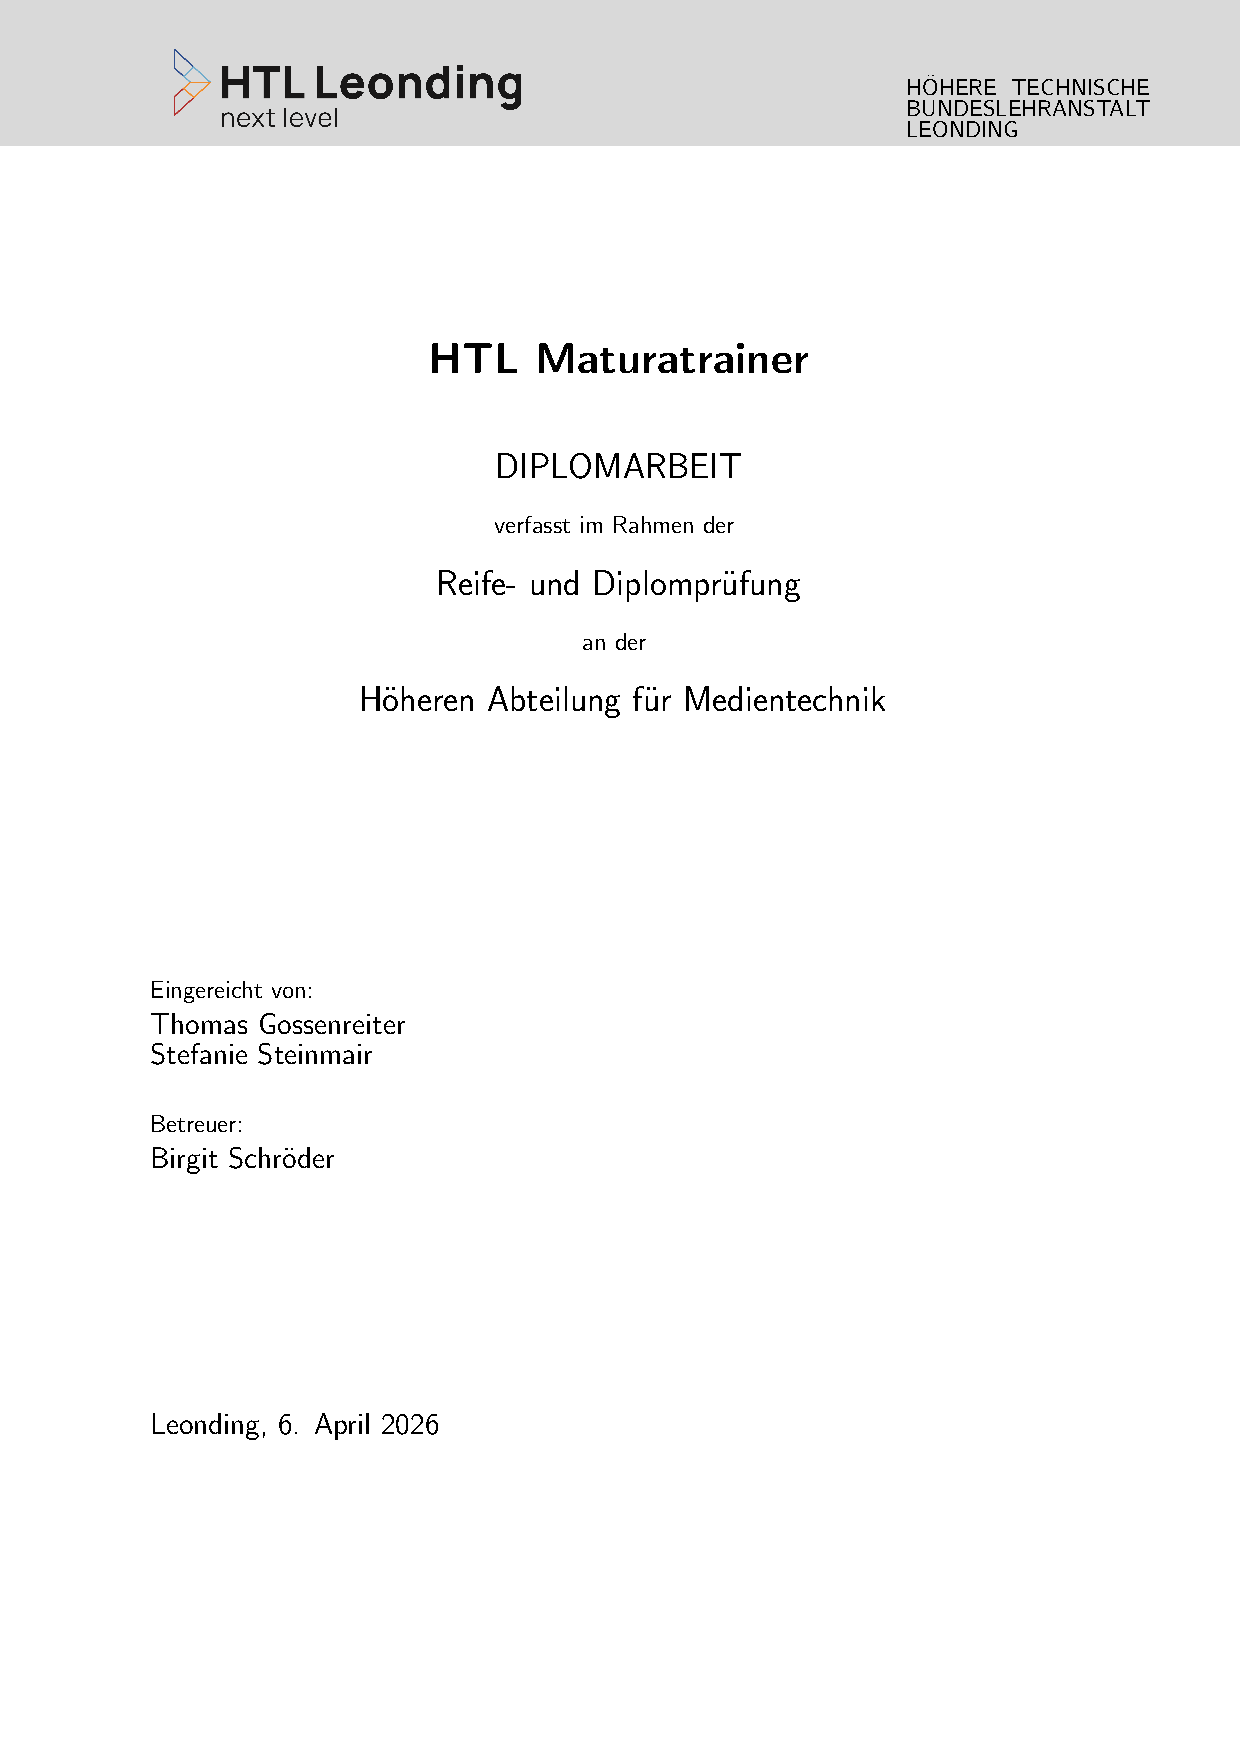
\includepdf{./titlepage/coversheet}
\pagenumbering{Roman}
\newpage
\thispagestyle{empty}
\vspace{3cm}
~ \\ \\
\IfStrEq{\thesislang}{de}
{
Ich erkläre an Eides statt, dass ich die vorliegende Diplomarbeit selbstständig und ohne fremde Hilfe verfasst, andere als die angegebenen Quellen und Hilfsmittel nicht benutzt bzw. die wörtlich oder sinngemäß entnommenen Stellen als solche kenntlich gemacht habe.

Die Arbeit wurde bisher in gleicher oder ähnlicher Weise keiner anderen Prüfungsbehörde vorgelegt und auch noch nicht veröffentlicht.

Die vorliegende Diplomarbeit ist mit dem elektronisch übermittelten Textdokument identisch.
}
{
I hereby declare that I have composed the presented paper independently and on my own, without any other resources than the ones indicated. 
All thoughts taken directly or indirectly from external sources are properly denoted as such.

This paper has neither been previously submitted to another authority nor has it been published yet.

The presented paper is identical to the electronically transmitted document.
}
\vspace{3cm}
% Hier kommt die Unterschrift drüber
\begin{tabbing}
Leonding, \IfStrEq{\thesislang}{de}{\duedatede}{\duedateen} \hspace{2cm} {\firstauthor} \& {\secondauthor} %, \thirdauthor \& \fourthauthor % replace & with , for all but the last author
\end{tabbing}
\vspace{10cm}
\newpage
\setcounter{page}{1}

\input{./sections/abstract}

\pagestyle{plain}

\IfStrEq{\thesislang}{de}
{
	\renewcommand{\lstlistlistingname}{Quellcodeverzeichnis}
}
{
 % keep at list of listing
}

\setcounter{tocdepth}{3}  % Subsubsections im TOC
\tableofcontents
\newpage
\setcounter{RPages}{\value{page}}
\setcounter{page}{0}
\pagenumbering{arabic}
\pagestyle{scrheadings}

\begin{spacing}{1}

% =========================
% Kapitel 1 – Einleitung
% =========================
\chapter{Einleitung}

\section{Ausgangslage}
\textit{Beschreibung der aktuellen Situation: Warum besteht Bedarf für die Matura-Lernplattform? Probleme beim Lernen, fehlendes Feedback, etc.}

\section{Motivation und Problemstellung}
\textit{Warum ist das Thema interessant und relevant? Hauptproblem, das gelöst werden soll.}

\section{Zielsetzung}
\textit{Was soll am Ende entstehen? Funktionen und Ziele der Plattform.}

\section{Grundlagen und Analyse}

\subsection{Marktanalyse}
\textit{Analyse bestehender Lernplattformen und digitaler Angebote.}

\subsubsection{StudySmarter}
\textit{Funktionsweise, Zielgruppe, Vorteile/Schwächen, Vergleich mit eigenem Projekt.}

\subsection{Anforderungen eines digitales Maturatraining}
\textit{Funktionale und nicht-funktionale Anforderungen.}

\subsection{Nutzen für Schüler:innen}
\textit{Mehrwert der Plattform: Motivation, individuelles Lernen, Feedback, Vorbereitung.}

\section{Lernstrategien}
\setauthor{\secondauthor}

\subsection{Leitner-System}
\textit{Karteikarten-Prinzip, Vorteile, Umsetzung im Projekt.}

\subsection{Spaced Repetition}
\textit{Verteiltes Lernen, Effektivität, Umsetzung digital.}

\subsection{Vergleich verschiedener Lernstrategien und Schlussfolgerung}
\textit{Leitner, Spaced Repetition, klassisches Lernen – Vor- und Nachteile - Ergebnis.}

% =========================
% Kapitel 2 – Technologische Entscheidungen
% =========================
\chapter{Technologische Entscheidungen und Architektur}

\section{Backend}
\textit{Backend-Aufbau}

\subsection{Datenbankstruktur}
\textit{Datenbanktabellen}

\subsection{Quarkus}
\textit{REST-Endpunkte, Speicherung von Feedback/Statistiken.}

\section{Frontend – Angular}

\subsection{Aufbau und Komponenten}
\textit{Struktur der App: Login, Dashboard, Übungsmodus, Prüfung, Ergebnisübersicht. Komponenteninteraktion.}

\section{Entwicklungsumgebung und Versionsverwaltung}
\textit{Verwendete Tools (IntelliJ, GitHub, Docker), Branching-Strategie, Teamwork.}

% =========================
% Kapitel 3 – Praktische Umsetzung
% =========================
\chapter{Praktische Umsetzung}

\section{Usecases}

\subsection{Üben}
\textit{User (Schüler) möchte für gezielte Themen für die Matura lernen.}
\textit{Usecase-Diagramme für User (Schüler) → Fragen beantworten, Feedback erhalten, eigenen Fragenpool erstellen}

\subsection{Prüfungssimulationen}
\textit{User (Schüler) möchte eine Prüfungssimulation starten, um sein Wissen zu testen.}
\textit{Usecase-Diagramme für User (Schüler) → Fragen beantworten, Feedback am Ende erhalten, Note erhalten}

\subsection{Fortschrittsübersicht}
\textit{User (Schüler) möchte seinen Lernfortschritt jederzeit einsehen und Statistiken betrachten.}
\textit{Usecase-Diagramme für User (Schüler) → Fortschritt (\% der unbeantworteten, falsch beantworteten, 1x, 2x, genug beantworteten Fragen), Durchschnittswertung bei Prüfungen usw.}

\section{Benutzeroberfläche und Design}

\subsection{Mockups und User Flow}
\textit{UI-Entwürfe (Figma), Nutzerführung Start → Übungsmodus → Ergebnis. Fokus auf Usability.}

% ------------------------------------------
% Use Case: Üben
% ------------------------------------------
\section{Use Case: Üben}

\subsection{Fragenhandling und Fragetypen}
\setauthor{\firstauthor}
\textit{Speicherung, Abruf, Darstellung verschiedener Fragetypen, Feedbacksystem.}

\subsection{Übungsmodus mit direktem Feedback}
\setauthor{\firstauthor}
\textit{Technische Umsetzung, Ablauf, User Experience.}

\subsection{Lösungswege und Nutzerinteraktion}
\setauthor{\secondauthor}
\textit{Einsehen von Lösungswegen, Feedbackmechanismen}

\subsection{Verwaltung von Fragenpools}
\setauthor{\secondauthor}
\textit{Auswahl eigener Fragen, Erstellung von individuellen Pools, Backend- und Frontend-Umsetzung.}

% ------------------------------------------
% Use Case: Prüfungssimulation
% ------------------------------------------
\section{Use Case: Prüfungssimulation}

\subsection{Prüfungsmodus mit Zeitlimit}
\setauthor{\firstauthor}
\textit{Simulation der Prüfung, Zeitlimit, realistische Prüfungssituation.}

\subsection{Bewertung und Ergebnisausgabe}
\setauthor{\firstauthor}
\textit{Ergebnisanzeige am Ende, Notenberechnung, Auswertung.}

% ------------------------------------------
% Use Case: Fortschritt
% ------------------------------------------
\section{Use Case: Fortschritt einsehen \& analysieren}

\subsection{Lernstrategien und Fehleranalyse}
\setauthor{\secondauthor}
\textit{Identifikation von Wiederholungsbedarf und Schwachstellen.}

\subsection{Spaced Repetition nach Leitner}
\setauthor{\secondauthor}
\textit{Technische Umsetzung der Lernstrategie, Speicherintervalle, Fortschrittslevel.}

\subsection{Lernstatistiken und Visualisierung}
\setauthor{\secondauthor}
\textit{Erhebung und grafische Darstellung der Daten zur Nutzerleistung. Bibliotheken und Darstellungskonzepte.}

\section{Usability-Test mit Mitschülern}
\textit{Testbeschreibung, Szenarien, Feedback, Umsetzung von Verbesserungen.}

\end{spacing}



\newpage
\pagenumbering{Roman}
\setcounter{page}{\value{RPages}}
\input{glossary}
\glsnogroupskiptrue
\IfStrEq{\thesislang}{de}
{
	\printglossary[title=Glossar,toctitle=Glossar]
}
{
	\printglossary[title=Glossary,toctitle=Glossary]
}
\spacing{1}{
\IfStrEq{\thesislang}{de}
{
	\bibliographystyle{ieeetrande}
}
{
	\bibliographystyle{IEEEtran}
}
\bibliography{bib}
}
\listoffigures
\listoftables
\lstlistoflistings
\appendix
\addchap{Anhang}
\input{./sections/appendix}
\end{document}

